\chapter{Experimentation \& Validation} \label{experimentationANDresults}
In this chapter we go through our Network setup and showcase the final implementation. This is a proof of concept implementation with its energy consumption and production functionality simulated.
As future work for this project, PowerChain could be tested against real world production and consumption data or even be implemented as a small scale energy trading network.

\section{Network Setup}
For our network setup, we created a virtual linux Ubuntu environment with the help of PROXMOX \cite{proxmox}.
We used this virtual environment to run our validator nodes. To setup the PowerChain network, we used the script pc\_CreateNetwork which we
created to be able to easily setup a bootnode and the required validator nodes. For our testing purposes, we created a network that submits blocks every second, with two validator nodes that
run on the same virtual environment. In a real life implementation, the different validators must be controlled by different systems and by different users to improve
decentralization. The more validator nodes a network has the better it will be in terms of decentralization. To visualize the block creation and transaction submissions 
to the network, we also setup the Ethereum Lite Explorer by Alethio.\cite{alethio} \\
\begin{figure}[h!]
    \centering
    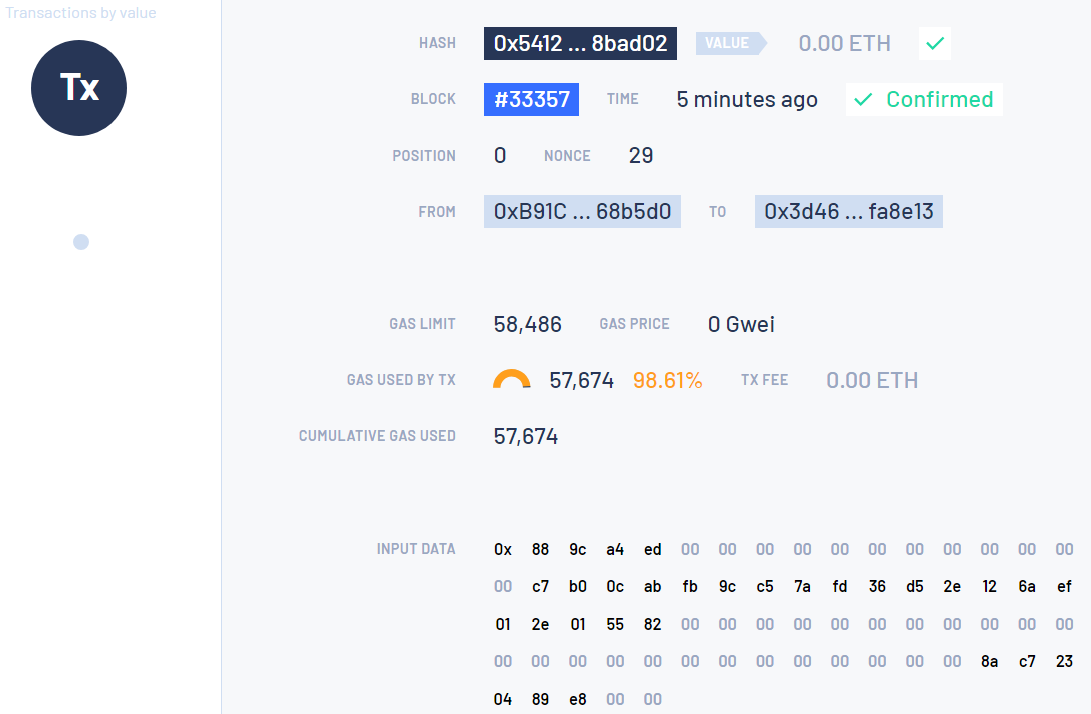
\includegraphics[width=\linewidth,frame,scale=0.9]{Figures/explorer.png}
    \caption{Example contract method execution transaction on blockchain explorer used with PowerChain}
\end{figure}
After the setup of the network, we need to deploy the PowerChain smart contract that contains all the decentralized functionality of our implementation.
To deploy the contract, we make use of the pc\_DeployContract script that is capable to deploy contracts in the blockchain network. The address that deploys the contract
is automatically given the voter role and is initially the only voter with the power to pass any votes by itself. As a first step for every PowerChain contract instance,
we need to add more voters in order to split the decision making and balance the interests of all parties involved. \\
The next step to finalize the network setup, is to deploy the PowerChain web application that will be used by the network users to interact with the smart contract. 
For our setup, we run the web application in the local network. We now have a working network with the PowerChain smart contract deployed on it and a web application running on
the local network to interact with the contract. The network parameters of the deployed PowerChain contract should have their default initial value (figure \ref{fig:initial_network_state}).
\begin{figure}[h!]
    \centering
    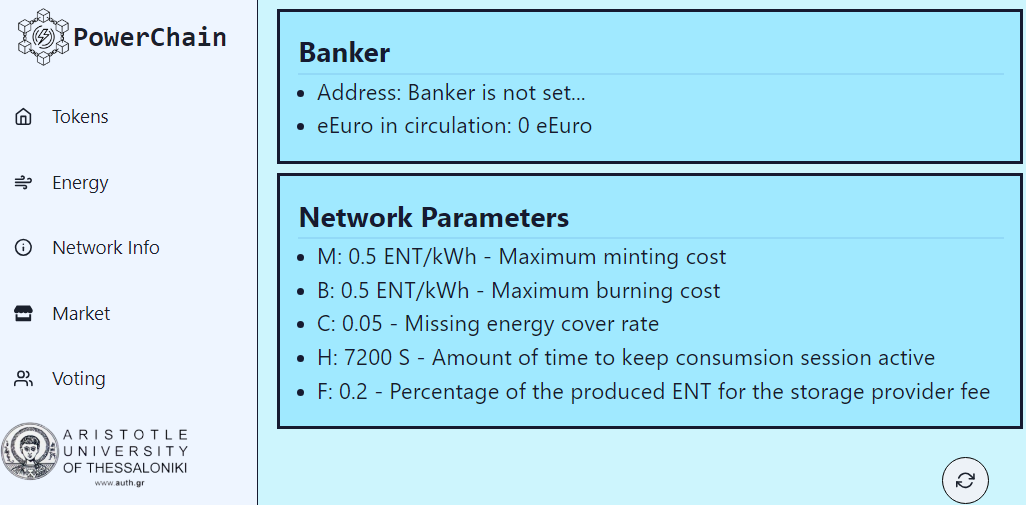
\includegraphics[width=\linewidth,frame,scale=1]{Figures/initial_network_state.png}
    \caption{Initial values for the PowerChain network parameters}
    \label{fig:initial_network_state}
\end{figure}


\section{Testing the PowerChain Contract}
To test the PowerChain contract, we constructed different energy trading scenarios and performed the relevant actions using the PowerChain web application.
Some of these test scenarios are presented in the following sections. Apart from the manual tests performed, we also created some jupiter notebooks that execute
pre-defined tests and checks the results automatically (refer to github address on chapter \ref{code}).

\section{Testing The Voting System}
For this test scenario, we go through the voting system of our PowerChain implementation and test its capabilities.
When the PowerChain contract is initially deployed the only voter in the network is the address that deployed the contract.
At this stage, this address has 100\% of the voting power and can execute any voter command immediately.\\
For this test, we created three blockchain network addresses: 
\begin{itemize}
    \item A = '0xb91ca997c40d6cf4c69ccd3f3c79bcc3ba68b5d0'
    \item B = '0xc7b00cabfb9cc57afd36d52e126aef012e015582'
    \item C = '0x80fc7a6634ea90774a21f43d51d2a84655ff3958'
\end{itemize}
The PowerChain contract is deployed by address A and thus A is automatically assigned the voter role.
As a first action, address A is executing the command 'Add Voter' to make address B a voter. This starts 
a voting procedure which is immediately passed and the action to make address B a voter is executed (figure \ref{fig:voter_added}).
\begin{figure}[h!]
    \centering
    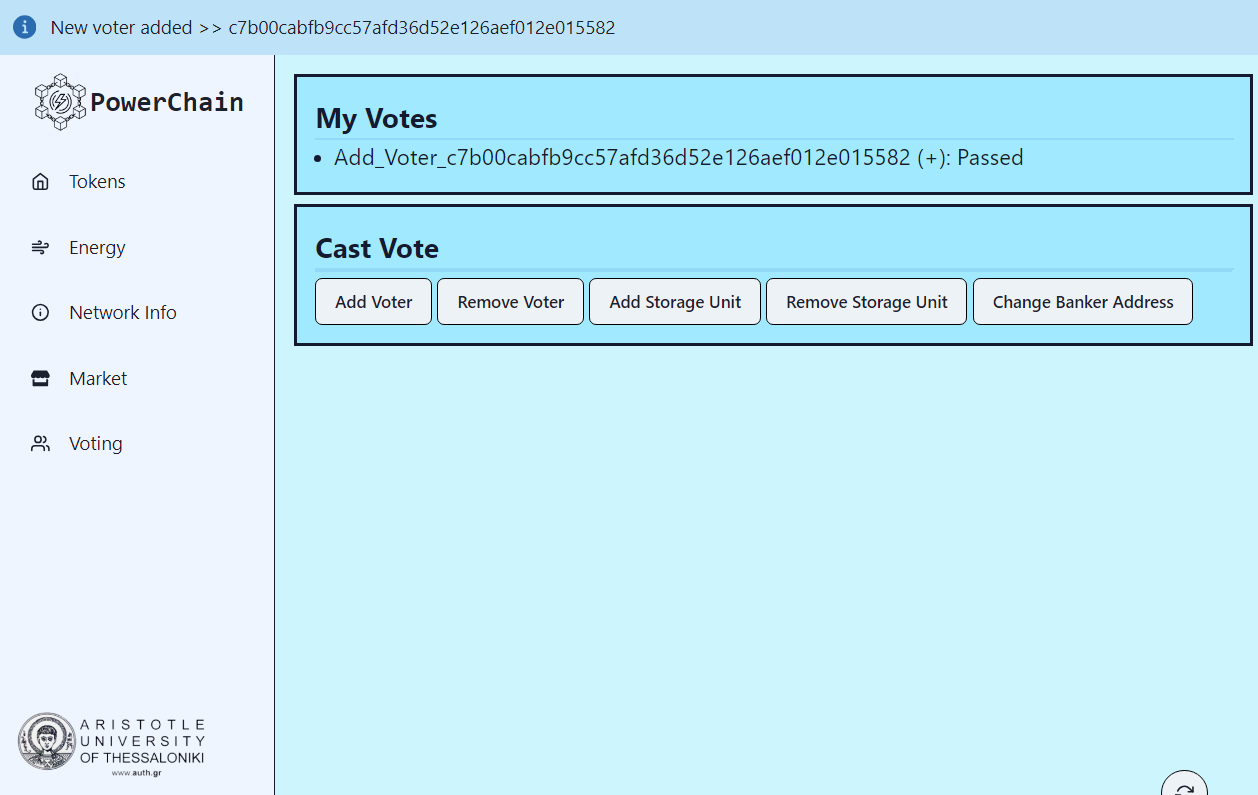
\includegraphics[width=\linewidth,frame,scale=0.7]{Figures/voter_added.png}
    \caption{Address A which has the voter role, assigns successfully the voter role to address B}
    \label{fig:voter_added}
\end{figure}
There are now two voters in the system, this means that in order to execute another voter command, both of them need
to agree. This is because the number of voters is now 2 and in order for the equation \ref{equ:vote_pass} to be valid,
we need at least 2 positive votes.\\
Next step is to also promote address C to a voter. Initially, address B executes the 'Add Voter' command to make address
C a voter but the action is not immediately executed, a voting procedure starts with one positive vote from address B (figure \ref{fig:add_voter_1}).
\begin{figure}[h!]
    \centering
    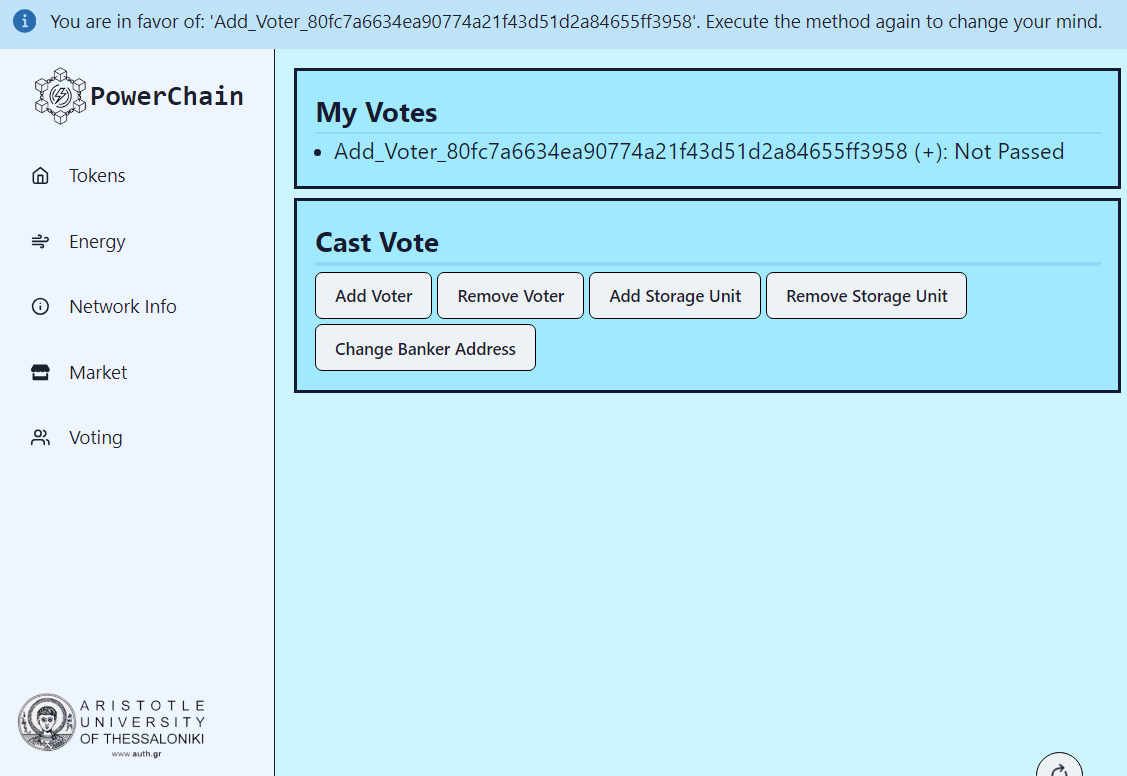
\includegraphics[width=\linewidth,frame,scale=0.7]{Figures/add_voter_1.png}
    \caption{Address B which is a voter, starts a voting procedure to add the voter role to address C}
    \label{fig:add_voter_1}
\end{figure}
Now it's time for address A to cast its positive vote by executing the command 'Add Vote' to give the voter
role to address C. This will make the voting to pass and the action to be actually executed which means that address C
will now be a voter (figure \ref{fig:add_voter_2}).\\
\begin{figure}[h!]
    \centering
    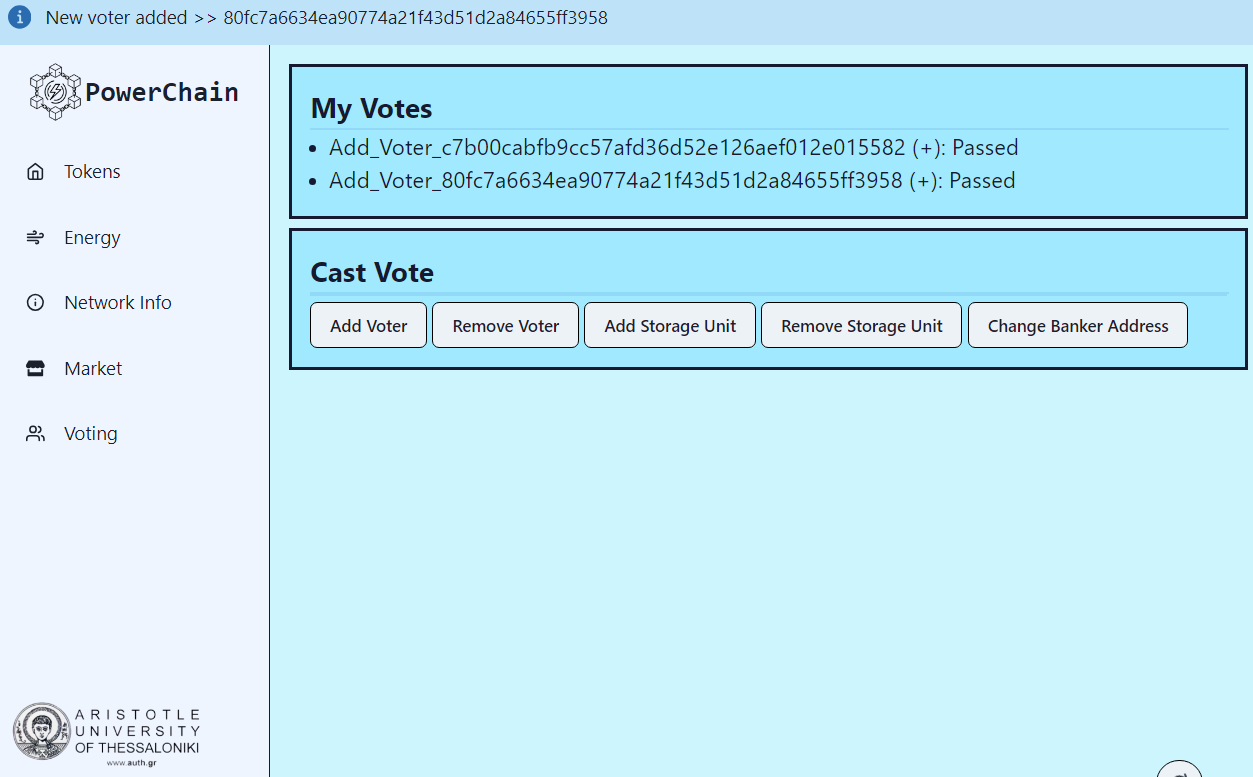
\includegraphics[width=\linewidth,frame,scale=0.7]{Figures/add_voter_2.png}
    \caption{Address A agrees on the voting to add the voter role to address C and the action is executed}
    \label{fig:add_voter_2}
\end{figure}
For the next step, we need to remove the voter role from address C. For this to happen at least two of the voters has to agree
on this action. Address A and B vote for the removal of address C from voters, the vote is passed and the voter role is revoked from address c (figure \ref{fig:remove_voter}).\\ 
\begin{figure}[h!]
    \centering
    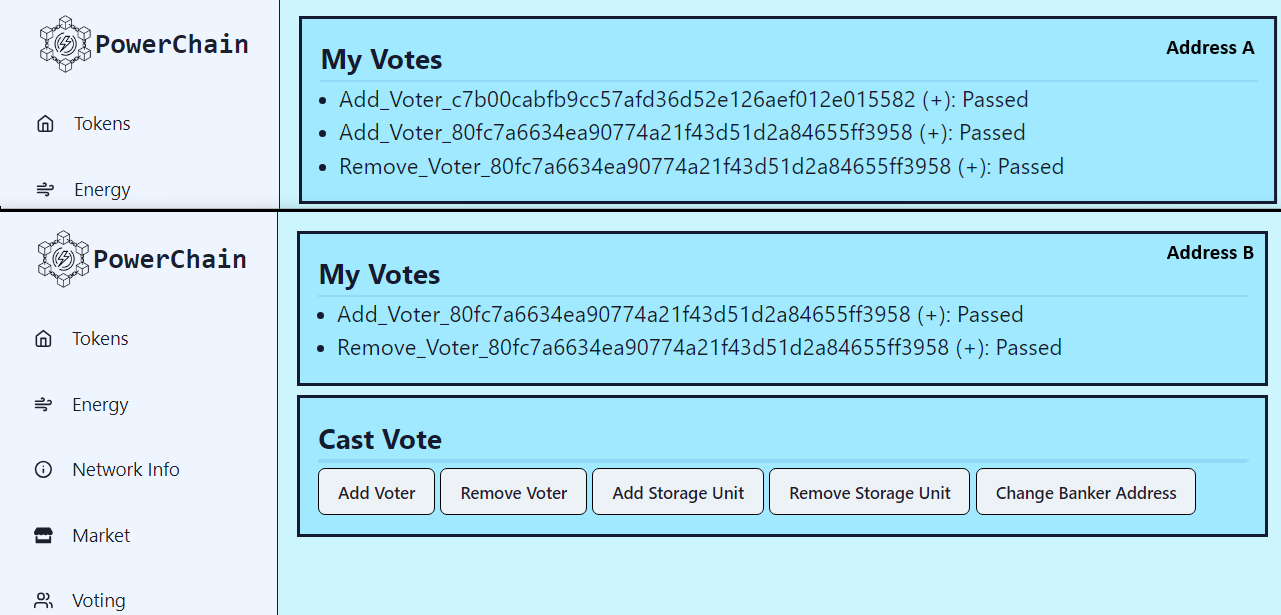
\includegraphics[width=\linewidth,frame,scale=0.7]{Figures/remove_voter.png}
    \caption{Address A and B which have the voter role, agrees to remove the voter role from address c and the action is executed}
    \label{fig:remove_voter}
\end{figure}
Concluding this testing scenario, we see that PowerChain smart contract protects important method executions that can impact the network significantly using
a voting system. Important network changes should be voted and agreed by most of the voters of the network. The voting system of PowerChain is handled automatically
by the smart contracts. This gives the voters freedom to execute commands that changes the network based on their believes. The changes are only truly performed if they 
are also agreed by most of the voters. \\

\section{Testing Energy Production And Consumption}
For this scenario, we will add two new storage units in the network and start producing and consuming energy.
For this purpose, we created the following blockchain addresses:
\begin{itemize}
    \item Voter Address A = '0xB91CA997C40D6CF4C69CCD3F3C79BCC3BA68B5D0'
    \item Voter Address B = '0xC7B00CABFB9CC57AFD36D52E126AEF012E015582'
    \item User Address C = '0x80FC7A6634EA90774A21F43D51D2A84655FF3958'
    \item Storage Unit Address U1 = '0x6E383425169CD23c3eb72709AEf8f81E7847310E'
    \item Storage Unit Address U2 = '0x16E36D7423AD7181B77818462fE0F5Ec5369aEb7'
\end{itemize}
We use the same setup from the previous scenario, so address A and B are already voters. As a first step, the addresses U1 and U2 need to be given the storage unit role to have the possibility to mint and burn
energy tokens (ENT) in the network based on the energy produced and consumed. To do so, voter A and voter B need to start two voting
sessions, one to give the address U1 the storage unit role and another one for U2. We will define as the owner of both storage units, the
user address C. As we only have two voter, both have to agree for the votes to pass (figure \ref{fig:add_units}).\\
\begin{figure}[h!]
    \centering
    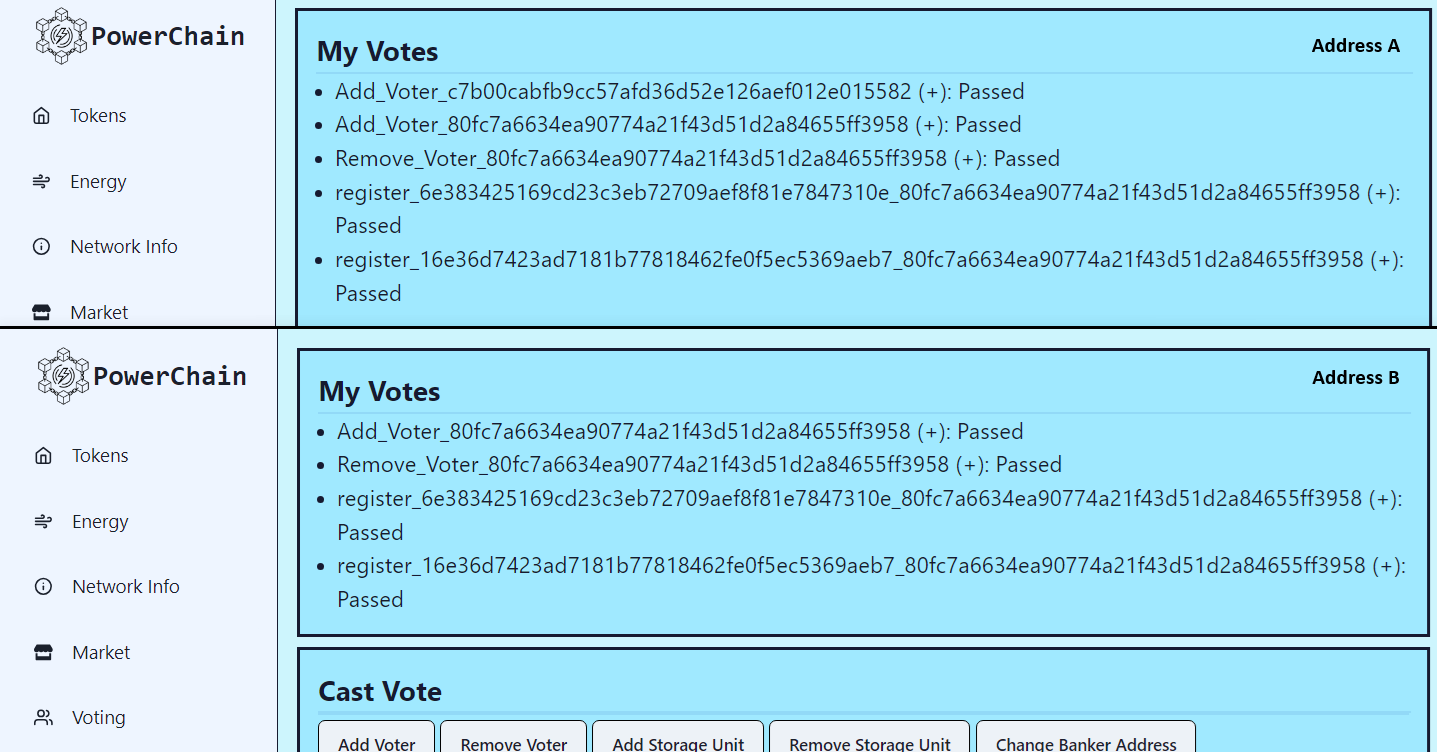
\includegraphics[width=\linewidth,frame,scale=1]{Figures/add_units.png}
    \caption{Address A and B which have the voter role, vote for the addition of two new storage units. The last two votes in the image represent the vote for the addition of the new storage units.}
    \label{fig:add_units}
\end{figure}
Now that we have two storage units in the network that are owned by user address C, the peer with address A, produces 10 kWh in the storage unit U1. The storage unit U1
reports the production to the blockchain and the relevant ENT tokens are minted. We simulate the energy production reporting using a python script (storage\_unit.py). In a real world scenario, there should be
a smart meter (an IoT device) that controls the storage unit address. This device is responsible to monitor the inbound/outbound energy and report relevant production and consumption of energy to the blockchain network.
After the production of 10 kWh from address A in the storage unit U1, address A should be rewarded with 8 ENT and the address C with 2 ENT. 
That's because the storage unit U1 belongs to user with address C and the storage provider fee parameter is set to 20\%.
As for the storage unit U1, it should now have 10 kWh available (figure \ref{fig:energy_produced}).\\
\begin{figure}[h!]
    \centering
    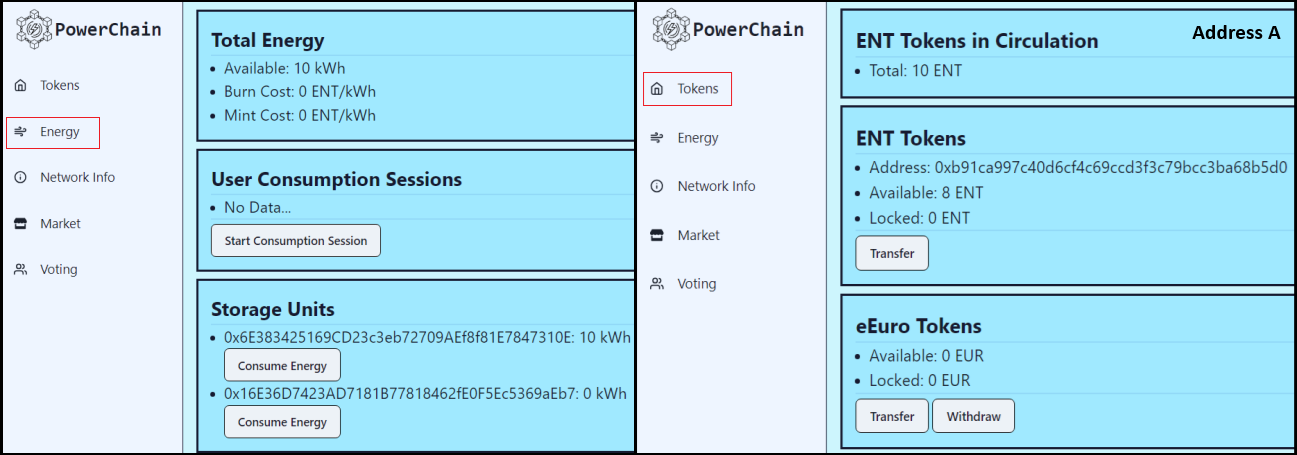
\includegraphics[width=\linewidth,frame,scale=1]{Figures/energy_produced.png}
    \caption{Overview of the web application information provided to address A after the energy production}
    \label{fig:energy_produced}
\end{figure}
For the next step, user with address C wants to consume some of the energy of storage unit U1. It has 2 ENT available which were received from the energy production of address A as a storage provider fee.
It starts a consumption session with unit U1 for 2 ENT which corresponds to an energy consumption of 2 kWh as there is no burn cost currently in the network.
With the consumption session of 2 kWh active, user address C consumes 1 kWh and unit U1 reports it. At this stage, user address C should have 1 locked ENT (the other one was consumed) and the storage unit U1
should have 8 kWh available, 1 already consumed and another one locked in the consumption session with user address c. The total ENT in circulation should be reduced to 9 and the same should happen also to the
total energy in the network (figure \ref{fig:consumption_session}).\\ 
\begin{figure}[h!]
    \centering
    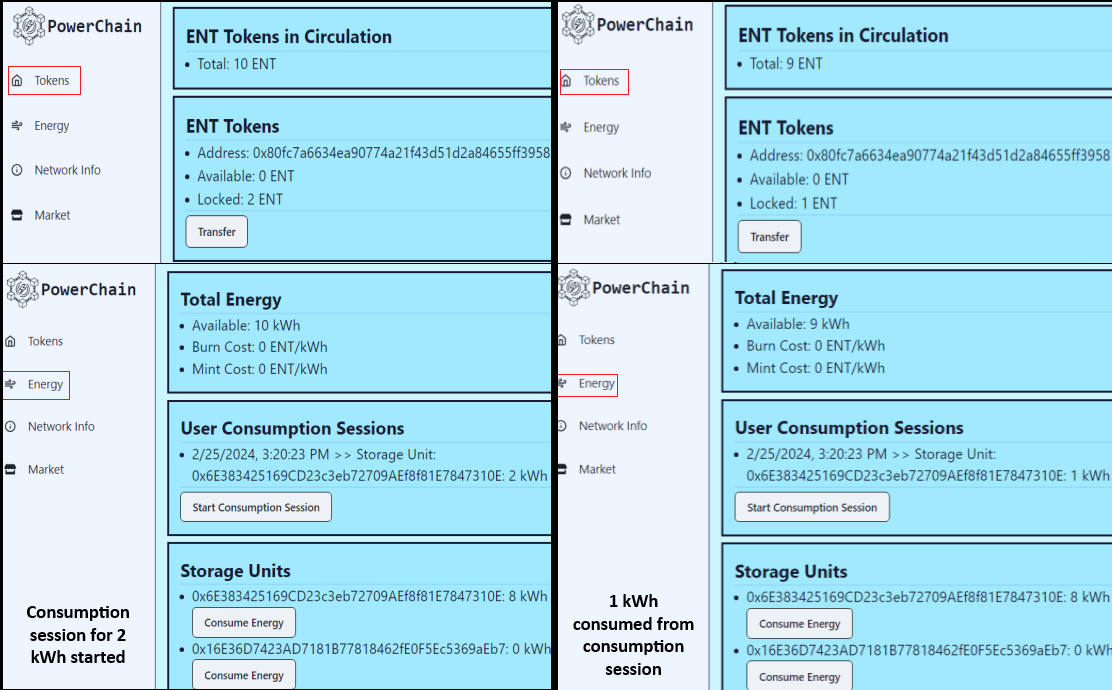
\includegraphics[width=\linewidth,frame,scale=1]{Figures/consumption_session.png}
    \caption{Consumption session of user address C before (left side) and after (right side) the consumption.}
    \label{fig:consumption_session}
\end{figure}
Proceeding further, we will study the case when the user address C consumes more kWh than were locked in the consumption session. This could happen due to an issue with the energy consumption monitoring of the smart
meter for example, which might allow the consumer to consume more than what was agreed with in the consumption session. In this case, we will have an imbalance in the system which will lead in a minting and burning
cost for the network, in order to counteract it. User address C has now 1 kWh left in the consumption session with unit U1 but due to a malfunction, 2 kWh were consumed. Unit U1 reports this consumption and the network will now have
8 ENT but only 7 kWh in total. The consumption session with user address C is terminated (figure \ref{fig:energy_imbalance}). \\
\begin{figure}[h!]
    \centering
    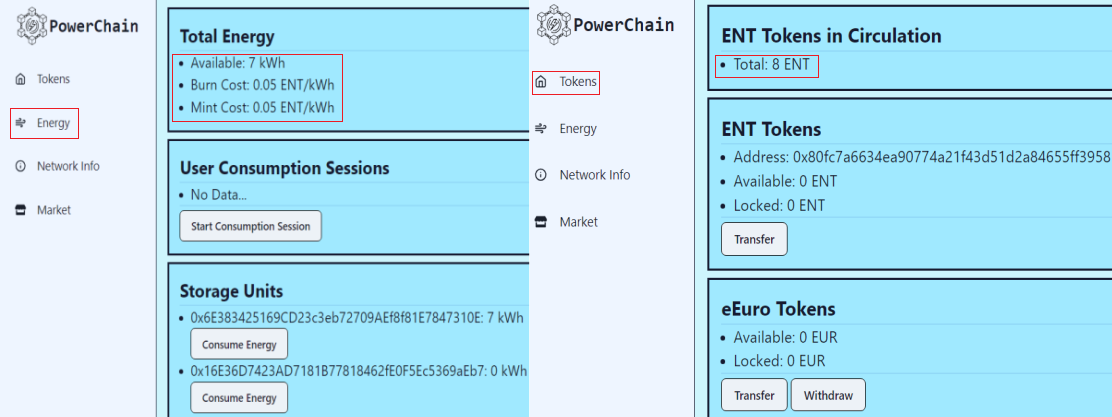
\includegraphics[width=\linewidth,frame,scale=1]{Figures/energy_imbalance.png}
    \caption{Due to network energy imbalance, a burning and minting cost is applied. The above image is an overview of the information provided to user address C.}
    \label{fig:energy_imbalance}
\end{figure}
The PowerChain smart contract will try to balance the ration between total ENT tokens and total kWh by applying a cost to each mint and burn of ENT tokens. Using the equation \ref{equ:kwh_until_equilibrium}, we can calculate when
equilibrium will be reached:
\begin{math}
    n_0 = \frac{D_0}{D_0*C} \Rightarrow n_0 = \frac{1}{C} \Rightarrow n_0 = 20 kWh
\end{math}.
So in the next 20 kWh that will be produced or consumed, the network will reach equilibrium. To study this behavior, we first produce 10 kWh from address B into storage unit U2.
This will reduce the difference to $D_{t1} = D_0 - 10*R \Rightarrow D_{t_1} = D_0 - 10*D_0*C \Rightarrow D_{t_1} = 0.5$. From this energy production $E_p$, the ENT tokens minted $\textrm{ENT}_{mint}$, based on the
minting cost $R=D_0*C=0.05$, are $\textrm{ENT}_{mint}=E_p*(1-R) \Rightarrow \textrm{ENT}_{mint}=10-10*0.05=9.5 ENT$. Due to the storage provider fee $F$, the ENT tokens received by
address B, are $\textrm{ENT} = \textrm{ENT}_{mint} - \textrm{ENT}_{mint} * F = 7.6 ENT$ (figure \ref{fig:reduce_imbalance}).\\
\begin{figure}[h!]
    \centering
    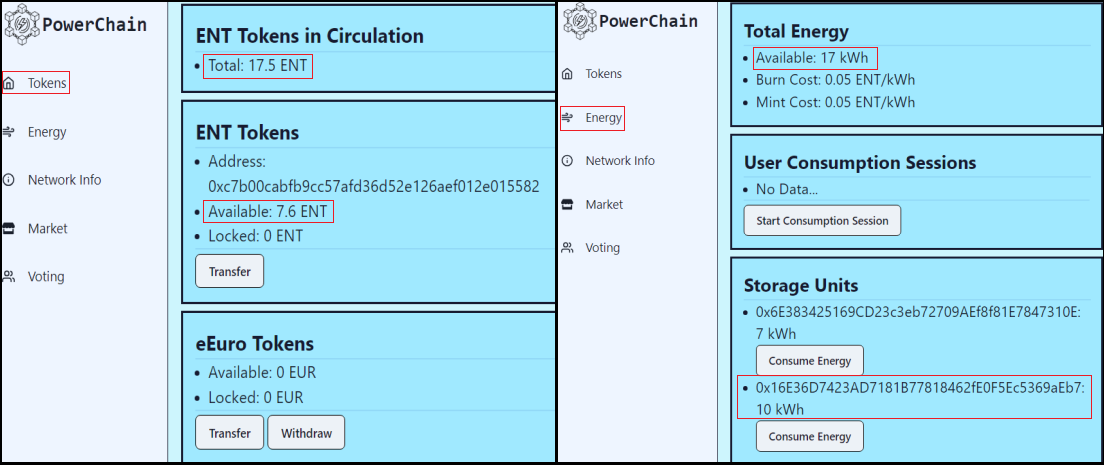
\includegraphics[width=\linewidth,frame,scale=1]{Figures/reduce_imbalance.png}
    \caption{After the production of 10kWh, the energy imbalance is reduced. In this figure we see the information provided to address B.}
    \label{fig:reduce_imbalance}
\end{figure}
As a final step for this scenario, we try to resolve the imbalance with an energy consumption worth of 15.6 ENT. To do so, address B transfers
its 7.6 ENT tokens to address A in order for address A to have 15.6 ENT available. Address A starts a consumption session for 7.35 ENT with unit U1 
and for 8.25 ENT with unit U2. Based on the burn cost, this is equivalent to $7.35/(1+R) = 7 kWh$ for the consumption session with unit U1 and 
$8.25/(1+R) = 7.857 kWh$ for the consumption session with unit U2. Address A consumes initially the 7 kWh from unit U1 and the storage unit reports the
consumption to the blockchain network. This will result in reduction of the difference between the total ENT and available energy to $D_{t_2} = D_0 - 17*R \Rightarrow 
D_{t_2} = D_0 - 17*D_0*C \Rightarrow D_{t_2} = 0.15$ (figure \ref{fig:reduce_imbalance_2}).
\begin{figure}[h!]
    \centering
    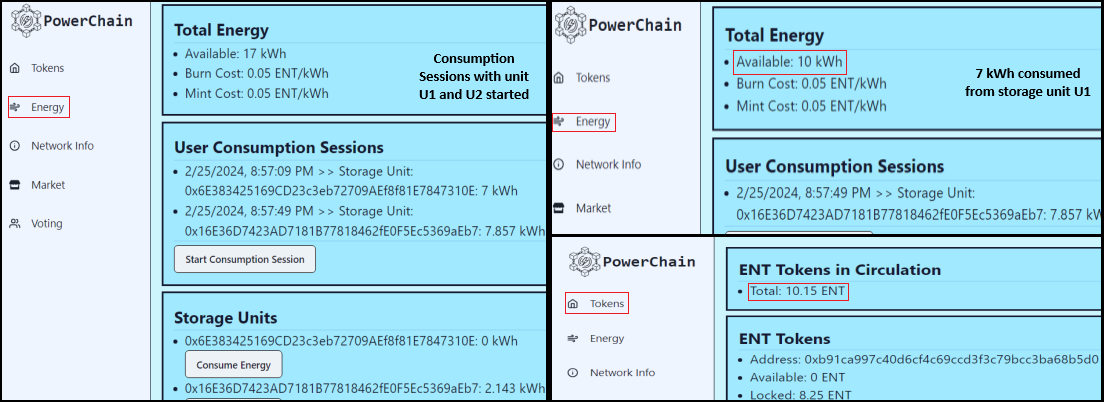
\includegraphics[width=\linewidth,frame,scale=1]{Figures/reduce_imbalance_2.png}
    \caption{Address A starts a consumption session with unit U1 and U2 (left side) and then consumes 7 kWh from storage unit U1 (right side).}
    \label{fig:reduce_imbalance_2}
\end{figure}
To cover the final difference $D_{t_2} = 0.15$ and reach equilibrium, we need to consume or produce another $n_{t_3} = \frac{D_{t_2}}{D_0*C} = 3 kWh$. To do
so, address A consumes the final 7.857 kWh from the consumption session with unit U2. From these 7.857 kWh, $E_e=3$ kWh will be consumed with ENT burning cost of 0.05 ENT/kWh
and the rest with no cost because after the 3 kWh, equilibrium will be reached and the cost $R$ will be set to 0. This means that the ENT to be burned from this energy
consumption are $\textrm{ENT}_{burn} = 3*(1+R) + (E_c-3) = 8.007 ENT$. For that reason $8.25 - 8.007 = 0.243 ENT$ will be returned back to address A because initially 8.25 ENT were
locked in this consumption session (figure \ref{fig:resolve_imbalance}). \\
\begin{figure}[h!]
    \centering
    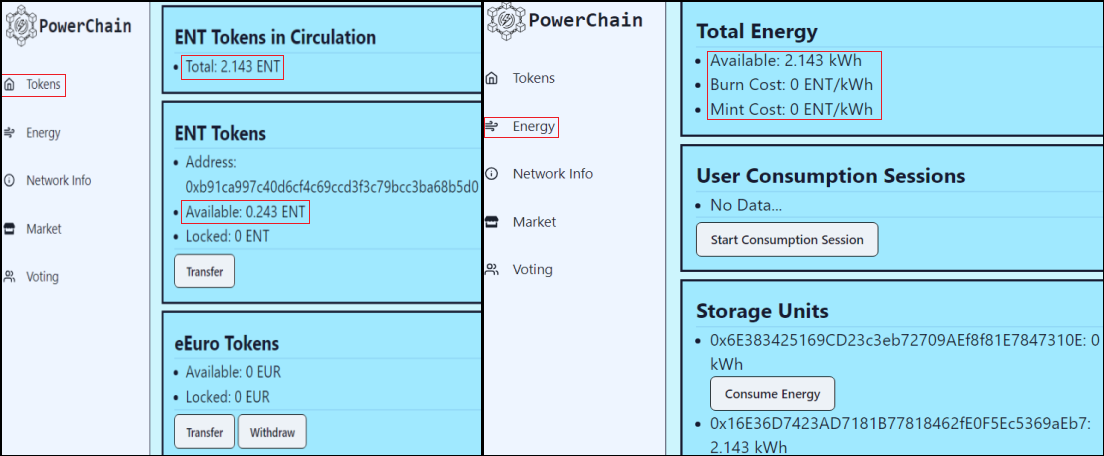
\includegraphics[width=\linewidth,frame,scale=1]{Figures/resolve_imbalance.png}
    \caption{This this figure we see the information provided to address A after the consumption of the energy from the consumption session with unit U1. The imbalance between the total
    ENT in circulation and the available kWh in the network is resolved.}
    \label{fig:resolve_imbalance}
\end{figure}
Concluding this test scenario, we see that the PowerChain smart contract is able to handle energy consumption deals between the network users and the storage units. It is also capable to automatically 
handle imbalances between the available energy in the network and the ENT in circulation, by applying a minting and burning cost. The automatic balancing mechanism is important to keep the ENT token 
tethered to the value of a particular amount of energy which is 1 kWh is our case.

\section{Testing the market layer}
In this testing scenario, we test the market layer of the PowerChain contract. For this test we use the same addresses with the previous testing scenario. In the current state of the network,
address A has 0.243 ENT tokens and address C has 1.9 ENT tokens. In order to use the market layer, we need to introduce the banker role in our network. The banker role will allow us to mint 
eEuro tokens that can be used to buy and sell ENT tokens. For this purpose, voter address A and voter address B agree on giving the banker role to address C (figure \ref{fig:new_banker}).
\begin{figure}[h!]
    \centering
    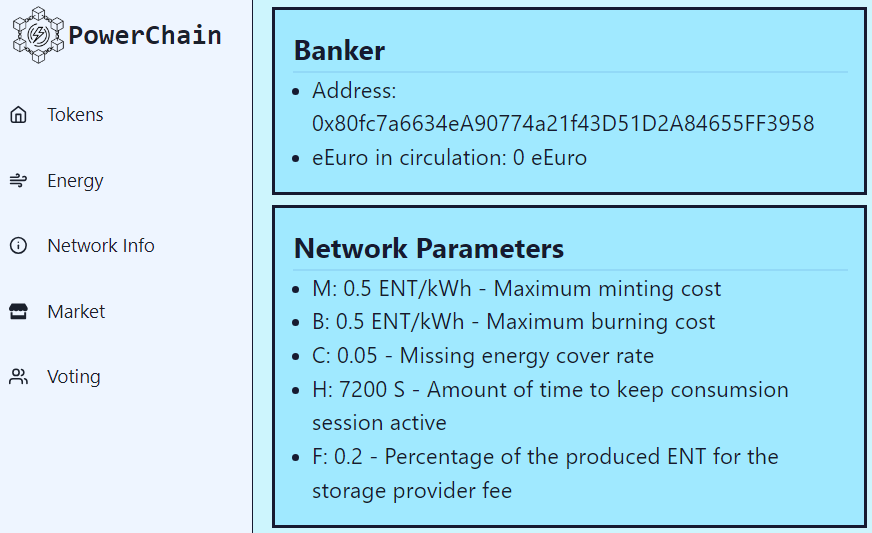
\includegraphics[width=\linewidth,frame,scale=0.7]{Figures/change_banker.png}
    \caption{In this figure we see the information provided to address A. The banker address has been changed to user address C.}
    \label{fig:new_banker}
\end{figure}
Address C can now move eEuro tokens in and out of circulation by minting and burning them. In a real world case, this role should be assigned to a trusted third party that will be responsible
to lock real world EUR and mint the relevant amount of eEuro in the PowerChain network. It is also responsible to unlock real world EUR and burn the relevant amount of eEuro, so the network users
can withdraw their eEuro. For the purposes of this test scenario, address C mints 10 eEuro into address A (figure \ref{fig:eEuro_minted}).\\ 
\begin{figure}[h!]
    \centering
    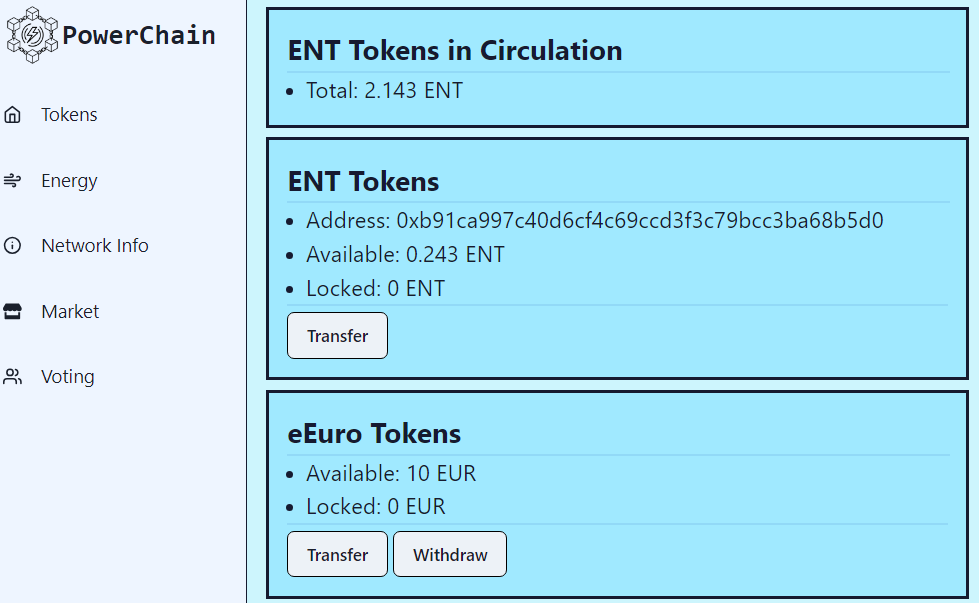
\includegraphics[width=\linewidth,frame,scale=0.7]{Figures/eEuro_minted.png}
    \caption{In this figure we see the information provided to address A. The banker address has been changed to user address C.}
    \label{fig:eEuro_minted}
\end{figure}
Address C has 1.9 ENT available and starts a sell order with cost 0.5 eEuro/ENT. Address A wants to buy 10 ENT with cost 1 eEuro/ENT and creates the relevant order in the market.
The system matches the buy order of address A with the sell order of address C and 1.9 ENT tokens are bought from address A for a total of 0.95 eEuro. This will reduce the requested
amount of the buy order of address A to 8.1 ENT with requesting price of 1 eEuro/ENT (figure \ref{fig:order_book}).\\ 
\begin{figure}[h!]
    \centering
    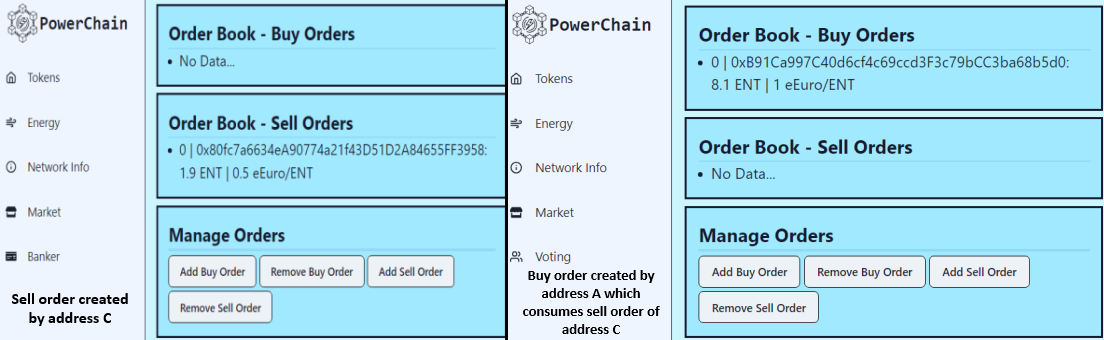
\includegraphics[width=\linewidth,frame,scale=1]{Figures/order_book.png}
    \caption{In this figure we can see the sell order created by address C (on the left side) and the buy order created by address A (on the right side) which automatically consumed the sell
    order of address C}
    \label{fig:order_book}
\end{figure}
Concluding this test scenario, we see that the PowerChain smart contract can automatically match the buy and sell orders of the users, using an order book style CDA market. This market maker mechanism
is very simplistic and could be enhanced to improve the user experience and possibly provide a unified energy price.

\section{Comparison with literature}
Based on our exterminations, it is apparent that PowerChain is a viable energy trading solution but how does it compare against the literature implementations we studied on chapter \ref{chapter3}?
In the following table we summarize the main aspects of the studied solutions along with our proposed one.
\newcolumntype{Y}{>{\centering\arraybackslash}m{2cm}}
\begin{table}[h!]
    \centering
    \begin{tabularx}{\textwidth}{|Y|Y|Y|Y|Y|Y|}
        \hline
        \textbf{Aspect}         & \textbf{PowerChain} & \textbf{\hyperref[sec:hfi]{A Frabric implementation}}      & \textbf{\hyperref[sec:dtr]{DeTrade}} & \textbf{\hyperref[sec:nrgc]{NRGCoin}} & \textbf{\hyperref[sec:cda]{Energy trading on CDA market}} \\
        \hline
        \textbf{Blockchain}     & Private Ethereum & Private Hyperledger Fabric & Private Hyperledger Burrow & Public Ethereum  & Public Bitcoin \\
        \hline
        \textbf{Consensus}      & PoA & BFT & BFT & PoS & PoW \\
        \hline
        \textbf{Market}         & Open Currency exchange with a CDA implementation on top & MCP (average buy offer) & DeMarket (pool-based) & Open currency exchange & CDA \\
        \hline
        \textbf{Energy Consumption} & Indirect, backed by ENT token & Direct, energy consumed at the time of production & Direct, energy consumed at the time of production & Indirect, backed by NRGCoin & Direct, energy consumed at the time of production \\
        \hline
        \textbf{Need for energy forecast} & No & Yes & Yes & No & Yes \\
        \hline
        \textbf{Relying on DSO and current energy transfer model} & Not if there is enough energy storage capacity in the network & Yes in case of energy contract breach due to forecast error & Yes in case of energy contract breach due to forecast error & Yes as it sends the produced energy to local substations & Yes in case of energy contract breach due to forecast error \\
        \hline
    \end{tabularx}
    \caption{Comparison of energy trading network from literature with PowerChain}
\end{table}\\ 
Compared to the models that follow a direct energy consumption architecture, approves upon the following points:
\begin{itemize}
    \item There is no need for energy forecasts giving the possibility to network participants to decide when and how much energy they need to consume or produce.
    \item There is no dependency on the traditional energy market and the DSOs as long as there is enough energy storage capacity on the network. Direct consumption approaches are always depended on the traditional energy market as there is always
    the risk of a forecast mistake which can lead to breaches to energy trading agreement and thus any excess energy produces or any additional energy consumption need to be covered by the traditional means.
    \item There is more freedom on when and how much energy to be consumed as the consumption and the production can happen asynchronously.
\end{itemize}
Compared to NRGCoin which uses the existing traditional energy transfer equipment to store energy, following an indirect energy consumption architecture, PowerChain introduces a local network energy storage layer. In that way, it decouples from the traditional energy
transfer model providing more freedom to its participants when it comes to how they want to maintain approve upon their network. Additional the energy market is formed only based on the participant needs and can't be immediately influenced by a DSO.

\section{Summarization}
In this chapter we examined our proof of concept PowerChain implementation by testing it against different scenarios. We tested the voting system of PowerChain by adding and removing voters in the network, the handling of energy consumption/production by the PowerChain
protocol and how an energy imbalance is handled automatically by the protocol through ENT minting and burning costs. We also tested the CDA energy trading market implemented in the PowerChain smart contract by creating some buying and selling orders of ENT tokens. Finally, we compared
the energy trading implementations of literature with our proposed solution and highlighted the points we are improving upon.